\title{Лекция 2\\Базовый язык представления знаний}   
\author[]{Шункевич Д.В.}
\institute[]{Белорусский государственный университет информатики и радиоэлектроники}

\begin{frame}
	\titlepage
\end{frame}

\begin{frame}{\\Содержание лекции}
	\topline
	\justifying
	Основные положения базового языка представления знаний в интеллектуальных системах – SC-кода.
	Алфавит, синтаксис, базовая денотационная семантика SC-кода.
	Синтаксическая и семантическая классификация sc-элементов.
\end{frame}

\begin{frame}{\\SC-code}
	\begin{SCn}
		\scnheader{SC-code} 
		\scnidtf{способ универсального смыслового представления (кодирования) информации в памяти компьютерных систем}
		\scnidtf{semantic computer code}
		\scnrelfrom{примечание}{SC-code основан на \textit{теории графов} (синтаксис) и \textit{теории множеств} (семантика), что обеспечивает универсальность и унифицированность (единообразие) представления информации, удобство машинной обработки и восприятия человеком}
	\end{SCn}
\end{frame}

\begin{frame}{\\Сравнение SC-code и двоичного кодирования}
	\vspace{10mm}
	\begin{textitemize}
		\item Двоичное кодирование
			\begin{textitemize}
				\item {алфавит \{0, 1\}}
				\item {не удобен для человека}
				\item {удобен для обработки в компьютере}
				\item {нельзя понять информацию без контекста}
				\item {легко реализовать}
			\end{textitemize}
		\item SC-code
			\begin{textitemize}
				\item {базовый алфавит состоит из 5 элементов}
				\item {удобен для человека}
				\item {удобен для обработки в компьютере}
				\item {обладает «осмысленностью»}
			\end{textitemize}
		\end{textitemize}
\end{frame}

\begin{frame}{\\Формы представления SC-кода}
	\vspace{10mm}
	\begin{SCn}
		\scnheader{SC-code}
		\scnidtf{абстрактный язык, который находится в памяти компьютерной системы}
		\scnrelfrom{примечание}{С помощью SC-кода можно описывать базы знаний, решатели задач и интерфейс интеллектуальной системы. SC-code является абстрактным языком, но его можно визуализировать в различных формах}
		\vspace{5mm}
		\textbf{Формы внешнего представления SC-кода}
			\begin{textitemize}
				\item {SCs-code (текстовый линейный)}
				\item {SCn-code (гипертекстовый)}
				\item {SCg-code (графический)}
			\end{textitemize}
	\end{SCn}
\end{frame}

\begin{frame}{\\}
	\vspace{5mm}
	\begin{columns}[T,onlytextwidth]
		\begin{column}{0.4\textwidth}
				\begin{SCn}
					\scnheader{SCs}
					\scnidtf{Semantic Code string}
					\scnidtf{язык линейного представления знаний}
					\scnheader{SCn}
					\scnidtf{Semantic Code natural}
					\scnidtf{язык структурированного представления знаний}
					\scnheader{SCg}
					\scnidtf{Semantic Code graphic}
					\scnidtf{язык графического представления знаний}
				\end{SCn}
		\end{column}
		\begin{column}{0.5\textwidth}
			\vspace{5mm}
			\begin{figure}[H]
				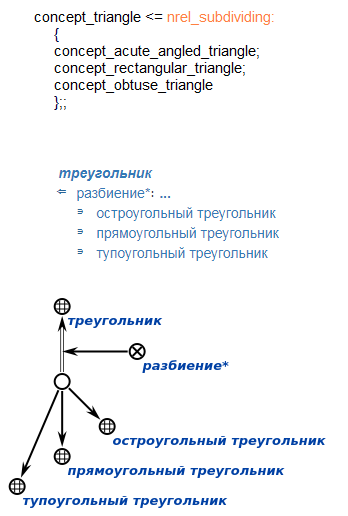
\includegraphics[scale=0.45]{./figures/sd_sc_code/ostis-basics-1.png}
			\end{figure}
		\end{column}
	\end{columns}
\end{frame}

\begin{frame}{\\Основные положения SC-code}
	\vspace{8mm}
	\begin{SCn}
		\scnheader{SC-code}
		\scnrelfrom{эпиграф}{Информация содержится не в самих знаках, а в конфигурации связей между ними}
		\scniselement{абстрактный язык}
		\scniselement{графовый язык}
		\begin{scnrelfromset}{основные положения}
			\scnitem{знаки сущностей --  синтаксически элементарные (атомарные) фрагменты sc-текстов, такие знаки не имеют внутренней структуры}
			\scnitem{информационные конструкции, не являющиеся sc-текстами, могут быть включены в базу знаний в виде файлов}
			\scnitem{тексты sc-кода имеют нелинейную (графовую) структуру, так как каждый знак сущности входит в базу знаний однократно и имеет неограниченное количество связей с другими знаками сущностей}
		\end{scnrelfromset}
	\end{SCn}
\end{frame}

\begin{frame}{\\}
	\begin{SCn}
		\scnheader{SC-code}
		\begin{scnrelfromset}{основные положения}
			\scnitem{база знаний (в виде текста SC-кода) является графовой структурой, алфавит элементов которой включает в себя множество узлов, рёбер, дуг, базовых дуг, а также множество специальных узлов, каждый из которых имеет содержимое, являющееся файлом, хранящимся в памяти интеллектуальной компьютерной системы}
			\scnitem{структурная особенность графовой структуры базы знаний заключается в том, что её дуги и ребра могут связывать не только узел с узлом, но и узел с ребром или дугой, ребро или дугу с другим ребром или дугой}
			\scnitem{отсутствие синонимии осуществляется благодаря склеиванию (отождествлению) одинаковых sc-элементов}
			\scnitem{sc-узлы, sc-ребра и sc-дуги являются обозначениями различных сущностей}
		\end{scnrelfromset}
	\end{SCn}
\end{frame}

\begin{frame}{\\SC-сущности}
	\vspace{7mm}
	\begin{SCn}
		\scnheader{ребро}
		\scnidtf{бинарная неориентированная связка}
		\scnheader{дуга}
		\scnidtf{бинарная ориентированная связка}
		\scnheader{базовая дуга}
		\scnidtf{связь между узлом (обозначающим некоторое множество элементов) и одним из элементов, который принадлежит указанному множеству}
		\scnheader{узел с содержимым}
		\scnidtf{файл}
	\end{SCn}
\end{frame}

\begin{frame}{\\}
	\begin{SCn}
		\scnheader{узел без содержимого}
		\scnidtf{материальный объект, первичный абстрактный
		объект, бинарная связь, множество и т.д.}
		\textbf{Пример узла без содержимого:}\\
		{Число, точка в некотором абстрактном пространстве}
		\scnheader{sc-сущности}
		\begin{scnrelfromset}{разбиение}
			\scnitem{постоянные (существуют всегда)}
			\scnitem{временные (им соотвествует отрезок времени их существования)}
			\scnitem{константные (конкретные)}
			\scnitem{переменные (произвольные)}
		\end{scnrelfromset}
	\end{SCn}
\end{frame}

\begin{frame}{\\}
	\begin{SCn}
		\scnheader{денотационная семантика языка}
	   	\scnidtf{семантические правила заданного языка}
	   	\scnheader{имя}
	   	\scnidtf{идентификатор, представляющий собой строку (цепочку) символов}
	   		\begin{scnrelfromset}{декомпозиция}
	   			\scnitem{простое имя}
	   			\begin{scnindent}
	   				\scnidtf{имя, в состав которого другие имена не входят, атомарное имя}
	   			\end{scnindent}
	   			\scnitem{выражение}
	   			\begin{scnindent}
	   				\scnidtf{неатомарное имя}
	   			\end{scnindent}
	   		\end{scnrelfromset}
	\end{SCn}
\end{frame}

\begin{frame}{\\Общие правила идентификации sc-элементов}
	\vspace{10mm}
	\begin{SCn}
		\begin{textitemize}
			\item если первым символом sc-идентификатора является знак подчеркивания, то идентифицируемый \textit{sc-элемент} принадлежит Классу sc-переменных (по умолчанию \textit{sc-элемент} принадлежит Классу sc-констант)
			\item если последним символом sc-идентификатора является символ ''звёздочка'', то идентифицируемый \textit{sc-элемент} принадлежит Классу обозначений неролевых отношений;
			\item если последним символом sc-идентификатора является апостроф, то идентифицируемый \textit{sc-элемент} принадлежит Классу обозначений ролевых отношений, каждое из которых является подмножеством Отношения принадлежности, то есть Класса всех константных позитивных пар принадлежности;
			\item если последним символом sc-идентификатора является символ ''\textasciicircum'', то идентифицируемый \textit{sc-элемент} принадлежит Классу обозначений параметров.
		\end{textitemize}
	\end{SCn}
\end{frame}

\begin{frame}{\\Семантическая классификация sc-элементов}
	К числу базовых признаков классификации \textit{sc-элементов} относятся:
	\begin{textitemize}
		\item структурный признак;
		\item логико-семантический признак;
		\item темпоральная характеристика сущностей, обозначаемых \textit{sc-элементами}, которая в свою очередь, включает в себя:
		\begin{textitemize}
			\item постоянство или временность существования обозначаемой сущности;
			\item статичность (стационарность) или динамичность (изменчивость) обозначаемой сущности.
		\end{textitemize}
	\end{textitemize}
\end{frame}

\begin{frame}{\\Структурная классификация sc-элементов}
	\vspace{10mm}
	\begin{SCn}
		\scnheader{sc-элемент}
		\scnrelfrom{разбиение}{Структурный признак классификации sc-элементов}
		\begin{scnindent}
			\begin{scneqtoset}
				\scnitem{обозначение sc-множества}
				\scnitem{обозначение внешней сущности}
				\begin{scnindent}
					\begin{scneqtoset}
						\scnitem{внутренний файл}
						\scnitem{внешняя сущность, не являющаяся внутренним файлом}
						\scnitem{обозначение файла}
						\scnitem{обозначение информационной конструкции, не являющейся ни sc-множеством, ни файлом}
						\scnitem{обозначение внешней сущности, не являющейся информационной конструкцией}
					\end{scneqtoset}
				\end{scnindent}
			\end{scneqtoset}
		\end{scnindent} 
	\end{SCn}
\end{frame}

\begin{frame}{\\}
	\vspace{10mm}
	\begin{SCn}
		\scnheader{обозначение sc-множества}
		\scnrelfrom{разбиение}{}
		\begin{scnindent}
		\begin{scneqtoset}
			\scnitem{обозначение sc-связки}
			\scnrelfrom{разбиение}{}
				\begin{scnindent}
				\begin{scneqtoset}
					\scnitem{обозначение sc-синглетона}
					\scnitem{обозначение sc-пары}
						\begin{scnindent}
						\begin{scneqtoset}
							\scnitem{обозначение неориентированной sc-пары}
							\scnitem{обозначение ориентированной sc-пары}
						\end{scneqtoset}
						\end{scnindent}
					\scnitem{обозначение sc-связки, не являющейся синглетоном и парой}
				\end{scneqtoset}
				\end{scnindent}
			\scnitem{обозначение sc-класса}
			\scnitem{обозначение sc-структуры}
		\end{scneqtoset}
		\end{scnindent}
	\end{SCn}
\end{frame}

\begin{frame}{\\}
	\begin{SCn}
		\scnheader{обозначение ориентированной sc-пары}
		\begin{scnindent}
			\begin{scneqtoset}
				\scnitem{обозначение sc-пары принадлежности}
				\begin{scnindent}
					\begin{scneqtoset}
						\scnitem{обозначение sc-пары нечеткой принадлежности}
						\scnitem{обозначение sc-пары позитивной принадлежности}
						\scnitem{обозначение sc-пары негативной принадлежности}
					\end{scneqtoset}
				\end{scnindent}
				\scnitem{обозначение ориентированной sc-пары, не являющейся парой принадлежности}
			\end{scneqtoset}
		\end{scnindent}
	\end{SCn}
\end{frame}

\begin{frame}{\\Логико-семантическая классификация}
	\vspace{5mm}
	\begin{SCn}
		\scnheader{sc-элемент}
		\begin{scneqtoset}
			\scnitem{sc-константа}
				\begin{scnindent}
				\scnidtf{sc-элемент, логико-семантическим значением которого является он сам}
				\end{scnindent}
			\scnitem{sc-переменная}
				\begin{scnindent}
				\begin{scneqtoset}
					\scnitem{sc-переменная 1-го уровня}
						\begin{scnindent}
						\scnidtf{sc-элемент, областью возможных значений которого является множество sc-констант}
						\end{scnindent}
					\scnitem{sc-переменная 2-го уровня}
						\begin{scnindent}
						\scnidtf{sc-элемент, возможными значениями которого являются переменные 1-го уровня}
						\end{scnindent}
					\scnitem{sc-переменная универсального типа}
						\begin{scnindent}
						\scnidtf{sc-переменная, на значения которой не накладывается никаких ограничений}
						\end{scnindent}
				\end{scneqtoset}
				\end{scnindent}
		\end{scneqtoset}	
	\end{SCn}
\end{frame}

\begin{frame}{\\Классификация темпоральная}
	\vspace{8mm}
	\begin{SCn}
		\scnheader{sc-элемент}
		\scnrelfrom{разбиение}{Признак постоянства существования сущностей, обозначаемых sc-элементами}
		\begin{scnindent}
			\begin{scneqtoset}
				\scnitem{обозначение постоянной сущности}
				\begin{scnindent}
					\scnidtf{обозначение постоянно существующей сущности}
				\end{scnindent}
				\scnitem{обозначение временной сущности}
				\begin{scnindent}
					\begin{scneqtoset}
						\scnitem{обозначение внешней временной сущности}
						\begin{scnindent}
							\scnsuperset{обозначение внешней ситуации}
							\scnsuperset{обозначение внешнего события}
							\scnsuperset{обозначение внешнего процесса}
						\end{scnindent}
						\scnitem{обозначение внутренней временной сущности}
						\begin{scnindent}
							\begin{scneqtoset}
								\scnitem{обозначение события в sc-памяти}
								\scnitem{обозначение инф. процесса в sc-памяти}
							\end{scneqtoset}
						\end{scnindent}
					\end{scneqtoset}
				\end{scnindent}
			\end{scneqtoset}
		\end{scnindent} 
		
	\end{SCn}
\end{frame}

\begin{frame}{\\}
	\vspace{10mm}
	\begin{SCn}
			Когда речь идёт о темпоральных свойствах sc-элементов, следует чётко отличать:
		\begin{textitemize}
			\item временный характер присутствия любого sc-элемента в составе той базы знаний, в которой он находится 
			\item временный характер присутствия в sc-памяти всей заданной sc-конструкции  (ситуации в sc-памяти);
			\item временный характер существования внешней сущности, которую sc-элемент обозначает;
			\item статичный (динам.) характер внешней сущности, обозначаемой sc-элементом; динамический характер внешней сущности, предполагает наличие в sc-памяти описания процесса изменения состояния или конфигурации указанной внешней сущности;
			\item динам. sc-множество, являющееся отражением соответствующего внешнего процесса;
			\item динам. sc-множество, являющееся отражением  соответствующего внутреннего процесса 
		\end{textitemize}
	\end{SCn}
\end{frame}

\begin{frame}{\\Структурная классификация sc-констант}
	\begin{SCn}
			Данная классификация полностью аналогична Структурной классификации sc-элементов, в отличие от которой она описывает структурную классификацию только константных sc-элементов (sc-констант) \\
			\scnheader{структурная классификация}
			\scniselement{sc-структура}
			\scnrelboth{аналог}{Структурная классификация sc-элементов}
	\end{SCn}
\end{frame}

\begin{frame}{\\}
	\begin{SCn}
		\scnheader{sc-константа}
		\begin{scneqtoset}
			\scnitem{sc-множество}
				\begin{scnindent}
				\begin{scneqtoset}
					\scnitem{sc-связка}
					\scnitem{sc-класс}
					\scnitem{sc-структура}
				\end{scneqtoset}
				\end{scnindent}
			\scnitem{внешняя сущность}
				\begin{scnindent}
					\scnidtf{sc-элемент, являющийся знаком внешней сущности}
					\scnidtf{знак внешней сущности}
					\scnidtf{знак сущности, не являющейся sc-множеством}
				\end{scnindent} 
			\begin{scnindent}
				\begin{scneqtoset}
					\scnitem{файл}
					\scnitem{внутренний файл}
					\scnitem{внешняя сущность (не внутренний файл)}
					\scnitem{внешняя сущность (не информационной конструкцией)}
					\scnitem{информационная конструкция (не sc-множество и не файл)}
				\end{scneqtoset}
			\end{scnindent}
		\end{scneqtoset}
		
	\end{SCn}
\end{frame}

\begin{frame}{\\}
	\begin{SCn}
		\scnheader{sc-связка}
			\begin{scnindent}
			\begin{scneqtoset}
				\scnitem{sc-синглетон}
				\scnitem{sc-пара}
					\begin{scnindent}
					\begin{scneqtoset}
						\scnitem{неориентированная sc-пара}
						\scnitem{ориентированная sc-пара}
						\scnitem{ориентированнная sc-пара, не являющаяся sc-парой принадлежности}	
						\end{scneqtoset}
						\end{scnindent}
				\scnitem{sc-связка, не являющаяся синглетоном и парой}
			\end{scneqtoset}
			\end{scnindent}
	\end{SCn}
\end{frame}

\begin{frame}{\\}
	\begin{SCn}
			\scnheader{ориентированная sc-пара}
			\begin{scnindent}
			\begin{scneqtoset}
				\scnitem{sc-пара принадлежности}
					\begin{scnindent}
					\begin{scneqtoset}
						\scnitem{sc-пара нечёткой принадлежности}
						\scnitem{sc-пара позитивной принадлежности}
						\scnitem{sc-пара негативной принадлежности}
					\end{scneqtoset}
					\end{scnindent}
				\scnitem{ориентированнная sc-пара, не являющаяся sc-парой принадлежности}	
			\end{scneqtoset}
			\end{scnindent}


	\end{SCn}
\end{frame}

